\subsection{Priors on Change-Point Locations}

\label{app:prior}

In the absence of any prior knowledge about the location of the change-point $\gamma \in [T]$, one natural choice is the uniform prior, $\pi_t = T^{-1}$. While this choice of $\boldsymbol{\pi}_{1:T}$ satisfies Assumption \ref{assumption:1} (iii) and therefore guarantees asymptotic consistency for each of the single change-point models in Section \ref{sec:scp}, the uniform prior may reduce detection power or even lead to false positives for small $T$. To see this we first show that the uniform prior does not induce a uniform posterior in the absence of a change-point. In Figure \ref{fig:post-probs-plot}, we plot MCMC estimates of $\E[\overline{\pi}_{1:T} \:|\: \mathbf{y}_{1:T}]$ for the three SCP models for a length $T=50$ univariate sequence $\mathbf{y}_{1:T}$ where $y_t \overset{\text{i.i.d.}}{\sim}\mathcal{N}(0,1)$. 
\begin{figure}[!h]
    \centering
    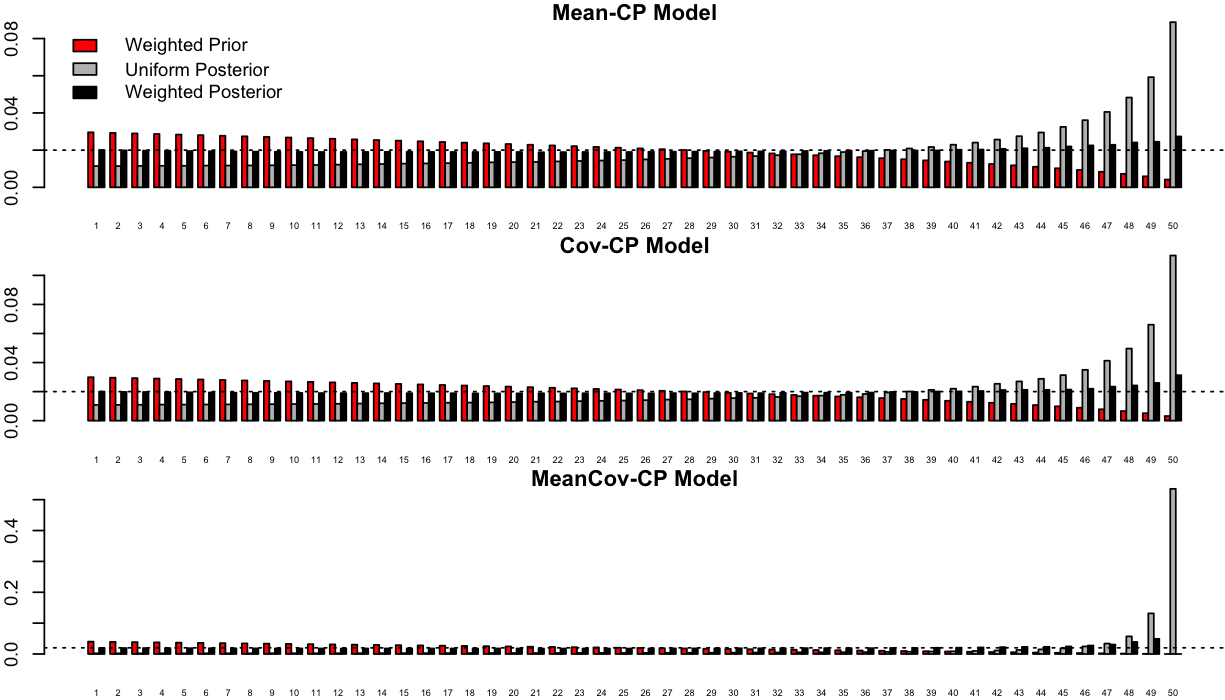
\includegraphics[scale = 0.4]{MICH/Figures/posterior_probs.png}
    \caption{$\E[\boldsymbol{\pi}_{1:T}\:|\: \mathbf{y}_{1:T}]$ under Null Model}
    \label{fig:post-probs-plot}
\end{figure}

Figure \ref{fig:post-probs-plot} shows an exponential increase in the posterior probabilities as $t$ approaches $T$. With a uniform prior, the SCP models may fail to detect a true change when the signal is weak or in small samples due to the large weight placed on times near $t = T$. For the cov-cp and meancov-cp models in particular, we see that the probabilities may be large enough to incorrectly detect a change-point in the vicinity of time $t=T$, even when no change is present. To rectify this behavior we propose selecting $\boldsymbol{\pi}_{1:T}$ so that when $\mathbf{y}_{1:T}$ is generated by the null model without a change-point, we have:
\begin{align}\label{eq:prior-cond}
    \E\left[\log\overline{\pi}_t - \log \overline{\pi}_{t+1} \right] = 0.
\end{align}
In Figure \ref{fig:post-probs-plot} we also plot the $\boldsymbol{\pi}_{1:T}$ that satisfies (\ref{eq:prior-cond}) and MCMC estimates of $\E[\overline{\pi}_{1:T} \:|\: \mathbf{y}_{1:T}]$ under this choice $\boldsymbol{\pi}_{1:T}$ so that (\ref{eq:prior-cond}) holds. We clearly see that these estimates adhere much more closely to the uniform dashed line at $T^{-1}$. Note that (\ref{eq:prior-cond}) also implies a uniform condition on the posterior probabilities since for any $r > t$:
\begin{align*}
    \E\left[\log\overline{\pi}_t - \log \overline{\pi}_r \right] &= \sum_{i=0}^{r-t-1} \E\left[\log\overline{\pi}_{t+i} - \log \overline{\pi}_{t+i+1} \right] = 0.
\end{align*}
We now proceed to show how to calculate $\pi_t$ so that (\ref{eq:prior-cond}) holds for each SCP model. For the mean-cp model in (\ref{eq:smcp-start})-(\ref{eq:smcp-end}) we have:
\small
\begin{align*}
    \E\left[\log\overline{\pi}_t - \log \overline{\pi}_{t+1} \right] &= \log \pi_t - \log \pi_{t+1} - \frac{1}{2} \log \left|\lambda_0\mathbf{I}_d + \sum_{t'=t}^{T} \boldsymbol{\Lambda}_{t'}\right| + \frac{1}{2} \log \left|\lambda_0\mathbf{I}_d + \sum_{t'=t+1}^{T} \boldsymbol{\Lambda}_{t'}\right|\\
    &\quad + \frac{1}{2} \E\left[\left\lVert \left[\lambda_0\mathbf{I}_d + \sum_{t'=t}^{T} \boldsymbol{\Lambda}_{t'}\right]^{-\frac{1}{2}} \sum_{t'=t}^{T} \boldsymbol{\Lambda}_{t'} \mathbf{y}_{t'}\right\rVert_2^2 \right]\\
    &\quad- \frac{1}{2} \E\left[\left\lVert \left[\lambda_0\mathbf{I}_d + \sum_{t'=t+1}^{T} \boldsymbol{\Lambda}_{t'}\right]^{-\frac{1}{2}} \sum_{t'=t+1}^{T} \boldsymbol{\Lambda}_{t'} \mathbf{y}_{t'}\right\rVert_2^2 \right].
\end{align*}
\normalsize
Letting $\lambda_0 \to 0$ and noting that $\sum_{t'=t}^{T} \boldsymbol{\Lambda}_{t'} \mathbf{y}_{t'} \sim \mathcal{N}_d\left(\mathbf{0}, \sum_{t'=t}^{T} \boldsymbol{\Lambda}_{t'}\right)$ under the null model, we get:
\small
\begin{align*}
    \E\left[\log\overline{\pi}_t - \log \overline{\pi}_{t+1} \right] &= \log \pi_t - \log \pi_{t+1} - \frac{1}{2} \log \left|\sum_{t'=t}^{T} \boldsymbol{\Lambda}_{t'}\right| + \frac{1}{2} \log \left|\sum_{t'=t+1}^{T} \boldsymbol{\Lambda}_{t'}\right|\\
    &\quad + \frac{1}{2} \E\left[\left\lVert \left[ \sum_{t'=t}^{T} \boldsymbol{\Lambda}_{t'}\right]^{-\frac{1}{2}} \sum_{t'=t}^{T} \boldsymbol{\Lambda}_{t'} \mathbf{y}_{t'}\right\rVert_2^2  \right] - \frac{1}{2} \E\left[\left\lVert \left[\sum_{t'=t+1}^{T} \boldsymbol{\Lambda}_{t'}\right]^{-\frac{1}{2}} \sum_{t'=t+1}^{T} \boldsymbol{\Lambda}_{t'} \mathbf{y}_{t'}\right\rVert_2^2  \right]\\
    &= \log \pi_t - \log \pi_{t+1} - \frac{1}{2} \log \left|\sum_{t'=t}^{T} \boldsymbol{\Lambda}_{t'}\right| + \frac{1}{2} \log \left|\sum_{t'=t+1}^{T} \boldsymbol{\Lambda}_{t'}\right|.
\end{align*}
\normalsize
If $\boldsymbol{\Lambda}_t = \boldsymbol{\Lambda}$ for all $t$, we can further simplify to:
\begin{align*}
    \E\left[\log\overline{\pi}_t - \log \overline{\pi}_{t+1} \right] &= \log \pi_t - \log \pi_{t+1} + \frac{d}{2} \log\left(\frac{T-t}{T-t+1}\right).
\end{align*}
Therefore, when (\ref{eq:prior-cond}) holds, we have a recurrence relation for writing $\log \pi_{t+1}$ in terms of $\log \pi_{t}$. It is without loss of generality to set $\log \pi_1 = 0$ in this relation since we can always normalize the sequence $\boldsymbol{\pi}_{1:T}$. 

For the cov-cp model in (\ref{eq:sscp-start})-(\ref{eq:sscp-end}) we have:
\small
\begin{align*}
    \E\left[\log\overline{\pi}_t - \log \overline{\pi}_{t+1} \right] &= \log \pi_t- \log \pi_{t+1} +\log \Gamma_d\left(\frac{u_0 + T-t+1}{2}\right) - \log \Gamma_d\left(\frac{u_0 + T-t}{2}\right) \\
    &\quad - \left(\frac{u_0 + T - t+1}{2}\right)\left(d\log 2 - \E\left[\log \left|v_0\mathbf{I}_d +  \sum_{t'=t}^{T} \boldsymbol{\Psi}^{\frac{1}{2}}_{t'}\mathbf{y}_{t'}\mathbf{y}^\intercal_{t'}\boldsymbol{\Psi}^{\frac{1}{2}}_{t'}\right| \right]\right) \\
    &\quad + \left(\frac{u_0 + T - t}{2}\right)\left(d\log 2 - \E\left[\log \left|v_0\mathbf{I}_d +  \sum_{t'=t+1}^{T} \boldsymbol{\Psi}^{\frac{1}{2}}_{t'}\mathbf{y}_{t'}\mathbf{y}^\intercal_{t'}\boldsymbol{\Psi}^{\frac{1}{2}}_{t'}\right| \right]\right) \\
    &\quad- \frac{1}{2}\sum_{t'=1}^{t-1} \E\left[\lVert\boldsymbol{\Psi}_{t'}^{\frac{1}{2}}\mathbf{y}_{t'}\rVert_2^2 \right] + \frac{1}{2}\sum_{t'=1}^{t} \E\left[\lVert\boldsymbol{\Psi}_{t'}^{\frac{1}{2}}\mathbf{y}_{t'}\rVert_2^2 \right].
\end{align*}
\normalsize
Letting $u_0 \to d-1$ and $v_0 \to 0$ and noting that $\mathbf{z}_{t} := \boldsymbol{\Psi}^{\frac{1}{2}}_{t'}\mathbf{y}_{t'} \sim \mathcal{N}_d\left(\mathbf{0}, \mathbf{I}_d\right)$ under the null model, we get:
\small
\begin{align*}
    \E\left[\log\overline{\pi}_t - \log \overline{\pi}_{t+1} \right] &= \log \pi_t- \log \pi_{t+1} +\log \Gamma_d\left(\frac{d + T-t}{2}\right) - \log \Gamma_d\left(\frac{d + T-t - 1}{2}\right) \\
    &\quad - \left(\frac{d+ T - t}{2}\right)\left(d\log 2 - \E\left[\log \left|\sum_{t'=t}^{T} \mathbf{z}_{t'}\mathbf{z}^\intercal_{t'}\right| \right]\right) + \left(\frac{d + T - t-1}{2}\right)\left(d\log 2 - \E\left[\log \left|\sum_{t'=t+1}^{T} \mathbf{z}_{t'}\mathbf{z}^\intercal_{t'}\right| \right]\right) \\
    &\quad- \frac{1}{2}\sum_{t'=1}^{t-1} d + \frac{1}{2}\sum_{t'=1}^{t} d
\end{align*}
\normalsize
When $T - t+ 1 > d - 1$, we have $\sum_{t'=t}^{T} \mathbf{z}_{t'}\mathbf{z}^\intercal_{t'} \sim \text{Wishart}(T-t+1, \mathbf{I}_d)$, so:
\begin{align*}
    \E\left[\log \left|\sum_{t'=t}^{T} \mathbf{z}_{t'}\mathbf{z}^\intercal_{t'}\right| \right] = \psi_d\left(\frac{T-t+1}{2}\right) + d\log 2
\end{align*}
where $\psi_d$ is the $d$-dimensional multivariate digamma function. For $t < T-d+1$ we now have:
\begin{align*}
    \E\left[\log\overline{\pi}_t - \log \overline{\pi}_{t+1} \right] &= \log \pi_t- \log \pi_{t+1} +\log \Gamma_d\left(\frac{d + T-t}{2}\right) - \log \Gamma_d\left(\frac{d + T-t-1}{2}\right) \\
    &\quad - \left(\frac{d + T - t}{2}\right)\psi_d\left(\frac{T-t+1}{2}\right) + \left(\frac{d + T - t-1}{2}\right)\psi_d\left(\frac{T-t}{2}\right) + \frac{d}{2}.
\end{align*}
If $T-t+1 \leq d-1$, then $\sum_{t'=t}^{T} \mathbf{z}_{t'}\mathbf{z}^\intercal_{t'}$  will be singular with probability one, but if we make the assumption that there is not change-point in the last $d-1$ time points, then we can satisfy (\ref{eq:prior-cond}) by setting $\pi_t = 0$ for $t \in \{T-d+2,\ldots,T\}$. So again we have defined a recursion for calculating $\pi_t$.

For the meancov-cp model in (\ref{eq:smscp-start})-(\ref{eq:smscp-end}) we have:
\scriptsize
\begin{align*}
    \E\left[\log\overline{\pi}_t - \log \overline{\pi}_{t+1} \right] &= \log \pi_t- \log \pi_{t+1} + \frac{d}{2}\log\left(\frac{T-t}{T-t+1}\right) +\log \Gamma_d\left(\frac{u_0 + T-t+1}{2}\right) - \log \Gamma_d\left(\frac{u_0 + T-t}{2}\right) \\
    &\quad - \left(\frac{u_0 + T - t+1}{2}\right)\left(d\log 2 - \E\left[\log \left|v_0\mathbf{I}_d +  \sum_{t'=t}^{T} \boldsymbol{\Psi}^{\frac{1}{2}}_{0}\mathbf{y}_{t'}\mathbf{y}^\intercal_{t'}\boldsymbol{\Psi}^{\frac{1}{2}}_{0}- \frac{1}{(\lambda_0 +T -t+1)^2} \left(\sum_{t'=t}^T \boldsymbol{\Psi}^{\frac{1}{2}}_{0}\mathbf{y}_{t'}\right)\left(\sum_{t'=t}^T \boldsymbol{\Psi}^{\frac{1}{2}}_{0}\mathbf{y}_{t'}\right)^{\intercal}\right| \right]\right) \\
    &\quad + \left(\frac{u_0 + T - t}{2}\right)\left(d\log 2 - \E\left[\log \left|v_0\mathbf{I}_d +  \sum_{t'=t+1}^{T} \boldsymbol{\Psi}^{\frac{1}{2}}_{0}\mathbf{y}_{t'}\mathbf{y}^\intercal_{t'}\boldsymbol{\Psi}^{\frac{1}{2}}_{0} - \frac{1}{(\lambda_0 +T -t)^2} \left(\sum_{t'=t+1}^T \boldsymbol{\Psi}^{\frac{1}{2}}_{0}\mathbf{y}_{t'}\right)\left(\sum_{t'=t+1}^T \boldsymbol{\Psi}^{\frac{1}{2}}_{0}\mathbf{y}_{t'}\right)^{\intercal} \right| \right]\right) \\
    &\quad- \frac{1}{2}\sum_{t'=1}^{t-1} \E\left[\lVert\boldsymbol{\Psi}_{0}^{\frac{1}{2}}\mathbf{y}_{t'}\rVert_2^2 \right] + \frac{1}{2}\sum_{t'=1}^{t} \E\left[\lVert\boldsymbol{\Psi}_{0}^{\frac{1}{2}}\mathbf{y}_{t'}\rVert_2^2 \right].
\end{align*}
\normalsize
Letting $u_0\to d-1$ and $\lambda_0,v_0 \to 0$ we get:
\small
\begin{align*}
    \E\left[\log\overline{\pi}_t - \log \overline{\pi}_{t+1} \right] &= \log \pi_t- \log \pi_{t+1} + \frac{d}{2}\log\left(\frac{T-t}{T-t+1}\right) +\log \Gamma_d\left(\frac{d + T-t}{2}\right) - \log \Gamma_d\left(\frac{d + T-t - 1}{2}\right) \\
    &\quad - \left(\frac{d + T - t}{2}\right)\left(d\log 2 - \E\left[\log \left|\left(\sum_{t'=t}^{T} (\boldsymbol{\Psi}^{\frac{1}{2}}_{0}\mathbf{y}_{t'} - \boldsymbol{\Psi}^{\frac{1}{2}}_{0}\overline{\mathbf{y}}_{t:T})(\boldsymbol{\Psi}^{\frac{1}{2}}_{0}\mathbf{y}_{t'} - \boldsymbol{\Psi}^{\frac{1}{2}}_{0}\overline{\mathbf{y}}_{t:T})^\intercal\right)\right| \right]\right) \\
    &\quad + \left(\frac{d + T - t-1}{2}\right)\left(d\log 2 - \E\left[\log \left|\left(\sum_{t'=t+1}^{T} (\boldsymbol{\Psi}^{\frac{1}{2}}_{0}\mathbf{y}_{t'} - \boldsymbol{\Psi}^{\frac{1}{2}}_{0}\overline{\mathbf{y}}_{(t+1):T})(\boldsymbol{\Psi}^{\frac{1}{2}}_{0}\mathbf{y}_{t'} - \boldsymbol{\Psi}^{\frac{1}{2}}_{0}\overline{\mathbf{y}}_{(t+1):T})^\intercal\right)\right| \right]\right) \\
    &\quad- \frac{1}{2}\sum_{t'=1}^{t-1} \E\left[\lVert\boldsymbol{\Psi}_{0}^{\frac{1}{2}}\mathbf{y}_{t'}\rVert_2^2 \right] + \frac{1}{2}\sum_{t'=1}^{t} \E\left[\lVert\boldsymbol{\Psi}_{0}^{\frac{1}{2}}\mathbf{y}_{t'}\rVert_2^2 \right]
\end{align*}
\normalsize
where $\overline{\mathbf{y}}_{t:T} = \frac{1}{T-t+1}\sum_{t'=t^T}\mathbf{y}_t$. Under the null model:
\begin{align*}
    \boldsymbol{\Psi}_0^{\frac{1}{2}}\mathbf{y}_t &\overset{\text{i.i.d.}}{\sim}\mathcal{N}_d(\mathbf{0},\mathbf{I}_d)
\end{align*}
and for $T-t>d-1$:
\begin{align*}
    \sum_{t'=t}^{T} (\boldsymbol{\Psi}^{\frac{1}{2}}_{0}\mathbf{y}_{t'} - \boldsymbol{\Psi}^{\frac{1}{2}}_{0}\overline{\mathbf{y}}_{(t+1):T})(\boldsymbol{\Psi}^{\frac{1}{2}}_{0}\mathbf{y}_{t'} - \boldsymbol{\Psi}^{\frac{1}{2}}_{0}\overline{\mathbf{y}}_{(t+1):T})^\intercal &\sim \text{Wishart}(T-t,\mathbf{I}_d).
\end{align*}
For the last result see Chapter 6.7 of \cite{Chatfield80} for reference.  For $t < T-d$ we now have:
\begin{align*}
    \E\left[\log\overline{\pi}_t - \log \overline{\pi}_{t+1} \right] &= \log \pi_t- \log \pi_{t+1} + \frac{d}{2}\log\left(\frac{T-t}{T-t+1}\right) +\log \Gamma_d\left(\frac{d + T-t}{2}\right) - \log \Gamma_d\left(\frac{d + T-t-1}{2}\right) \\
    &\quad - \left(\frac{d + T - t}{2}\right)\psi_d\left(\frac{T-t}{2}\right) + \left(\frac{d + T - t-1}{2}\right)\psi_d\left(\frac{T-t-1}{2}\right) + \frac{d}{2}
\end{align*}
and again we can get a recursion for calculating $\pi_t$ by making the assumption that there is not change-point in the last $d$ time points and satisfy (\ref{eq:prior-cond}) by setting $\pi_t = 0$ for $t \in \{T-d+1,\ldots,T\}$.


In Figure , we plot the resulting prior probabilities for the case of $y_t \overset{\text{i.i.d.}}{\sim}\mathcal{N}(0,1)$. Furthermore, in Figure we have also plotted the posterior probabilities that result from using the sequence $\pi_{1:T}$ that satisfies (\ref{eq:prior-cond}) for each model. We see that these posterior probabilities are much closer to being uniform in the absence of a change-point. 

We can also show that the priors that satisfy (\ref{eq:prior-cond}) also satisfy Assumption \ref{assumption:1} (iii) in finite dimensions, and thus the Assymptotic analysis in Section \ref{sec:localization} is still valid for these choices of $\boldsymbol{\pi}_{1:T}$. For the mean-cp prior under the conditions of Theorem \ref{theorem:smcp}, for $j > 0$ we have:
\begin{align*}
    \log\frac{\pi_{t_0}}{\pi_{t_0+j}} = \frac{d}{2} \log\left(\frac{T-t_0 - j +1}{T - t_0 +1}\right)
\end{align*}
and:
\begin{align*}
    \log\frac{\pi_{t_0}}{\pi_{t_0-j}} = \frac{d}{2} \log\left(\frac{T-t_0 + j +1}{T - t_0 +1}\right)
\end{align*}
We have:
\begin{align*}
    -\frac{d}{2}\log T \leq -\frac{d}{2} \log\left(T - t_0 +1\right) \leq \frac{d}{2} \log\left(\frac{T-t_0 - j +1}{T - t_0 +1}\right) \leq 0
\end{align*}
and: 
\begin{align*}
    \frac{d}{2}\log T \geq \frac{d}{2} \log\left(T - t_0 + j +1\right) \geq \frac{d}{2} \log\left(\frac{T-t_0 + j +1}{T - t_0 +1}\right) \geq 0
\end{align*}
so $\log \frac{\pi_{t_0}}{\pi_t} = \mathcal{O}(d\log T)$.